\subsubsection{Quick Sort}
While performing the sort the algorithm, it also stores the state in steps. This is done for the solution checker to be able to check if the student has drawn the correct answer when simulating the quicksort algorithm.
\begin{itemize}
    \item Initial: The initial step is stored before the sorting starts. It contains a copy of the unsorted array.
    \item Split: The split step is stored each time the algorithm splits a list; it stores the unsorted list, the pivot point, left and right list.
    \item Merge: The merge step is stored each time the algorithm merges the sorted lists and pivot point. It stores information about the sorted left and right list, the pivot point and the sorted list after the merge.
\end{itemize}
\begin{figure}[H]
    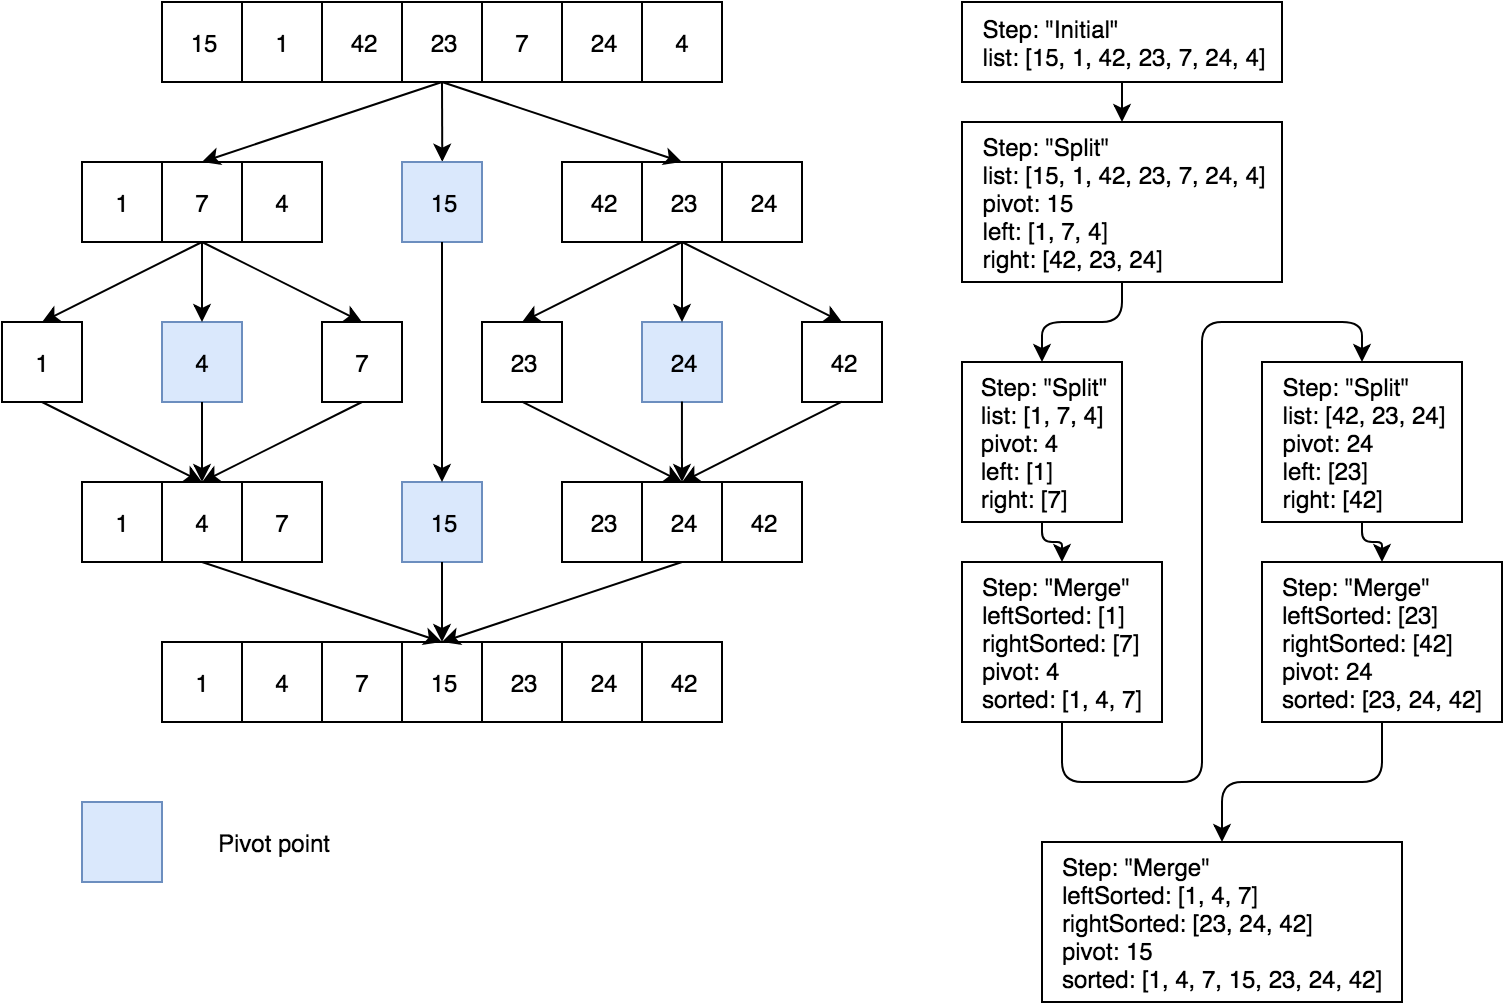
\includegraphics[width=\linewidth]{/diagrammer/Quicksort}
    \caption{Quicksort}
    \label{fig:quicksort}
\end{figure}